\section{Autopilot Design}
\subsection{}
The first order Nomoto model is a simple vessel model that we can use for this problem. The transfer function from rudder angle $\delta$ to heading rate $r = \dot \psi$ is given by equation (7.28) in \cite{Fossen2011} and is
\begin{equation}\begin{aligned}
\label{eq:nomoto_tf}
\frac{r}{\delta}(s) = \frac{K}{Ts + 1}
\end{aligned}\end{equation}
This corresponds to the time-domain representation
\begin{equation}\begin{aligned}
T \ddot \psi + \dot \psi = K \delta.
\end{aligned}\end{equation}

\subsection{}
In order to find the Nomoto parameters $T$ and $K$, we look at the step response of the system when excited by a reference $\delta_{\text{max}} = -25^{\circ}$, i.e. the maxiumum allowed rudder angle. Solving \eqref{eq:nomoto_tf} for the step response $r(t)$ we find
\begin{equation}\begin{aligned}
r(t) = \delta_{\text{max}} KT(1 - e^{-\frac{t}{T}}).
\end{aligned}\end{equation}
From classic control theory, we know that when $t = T$, $1 - e^{-\frac{t}{T}} = 1 - e^{-1} \approx 0.63$. In other words, the step response will hit $63\%$ of the final heading rate value $r_{\infty}$ at $t = T$. From \figref{fig:nomoto_reading} we see that this is at approximately $t = 140s$. Furthermore, as time goes to infinity, the exponential term goes to zero, and so $r$ approaches $\delta_{\text{max}} K T$. We read $r_\infty \approx 6.5 \cdot 10^{-3}$ from \figref{fig:nomoto_reading} and can then find $K$ as
\begin{equation}\begin{aligned}
K = \frac{r_{\infty}}{\delta_{\text{max}} T} \approx \frac{6.5 \cdot 10^{-3}}{25^{\circ} \cdot 140} \approx 1.06 \cdot 10^{-4}.
\end{aligned}\end{equation}
In total, we define the parameters
\begin{equation}\begin{aligned}
T = 140, \quad \text{and} \quad K = 1.06 \cdot 10^{-4}.
\end{aligned}\end{equation}

\begin{figure}[H]
\centering
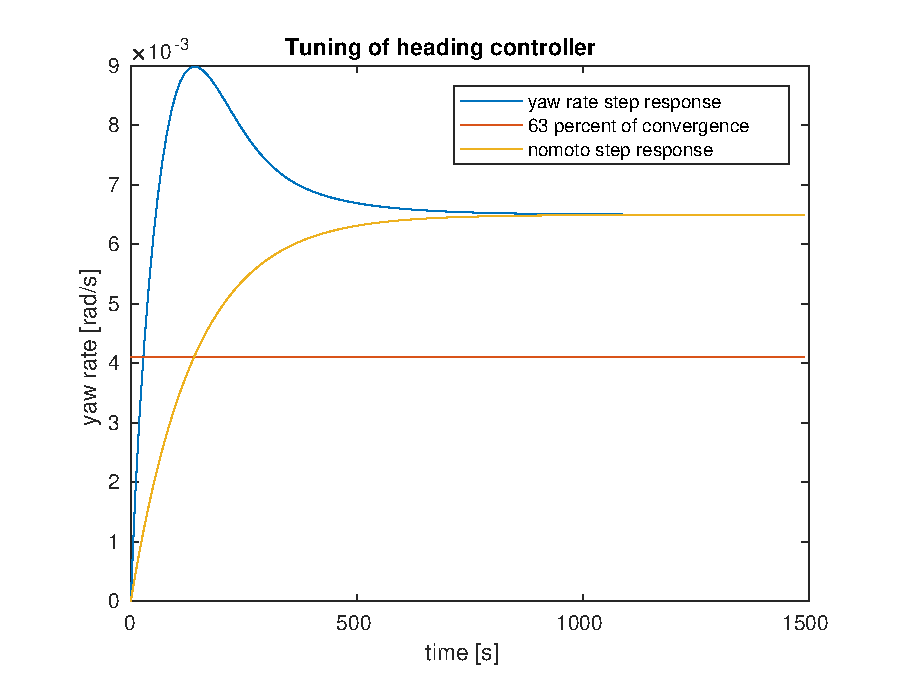
\includegraphics[width=0.7\textwidth]{nomoto-reading-improved}
\caption{Nomoto model parameter reading}
\label{fig:nomoto_reading}
\end{figure}


\subsection{}
We define a PD controller to control the heading $\psi$ from the rudder, i.e. we want the commanded rudder to be
\begin{equation}\begin{aligned}
\delta_c = -K_p (\psi_d - \psi) - K_d \psi_dot.
\end{aligned}\end{equation}
We wish to use the Nomoto model to find good values for $K_p$ and $K_d$. Using the model parameters, we define
\begin{equation}\begin{aligned}
T' = T \frac{U}{L_{pp}}, \quad K' = K \frac{L_{pp}}{U},
\end{aligned}\end{equation}
where $U = \sqrt{u^2 + v^2}$ is the ship velocity and $L_{pp}$ is the ship length. We also define
\begin{equation}\begin{aligned}
\omega_n = \sqrt{(\frac{u}{L_{pp}}) (\frac{1}{T})}, \quad \text{and} \quad \xi = 1.
\end{aligned}\end{equation}
With this, we choose the controller parameters
\begin{equation}\begin{aligned}
K_p = (\frac{L_{pp}}{U})^2 \frac{T'}{K'}, \quad \text{and} \quad
K_d = \frac{2 \xi \omega_n - 1}{K' \frac{U}{L_{pp}}}.
\end{aligned}\end{equation}
Since this control input will be input into a physical rudder, we have to saturate $\delta_c$ between the minimum and maximum rudder angles $-\delta_{\text{max}}$ and $\delta_{\text{max}}$. In addition, we could add rate limitation to the input, but we have not implemented this.



\begin{figure}[ht]
	\centering
	\begin{subfigure}[b]{0.45\textwidth}
		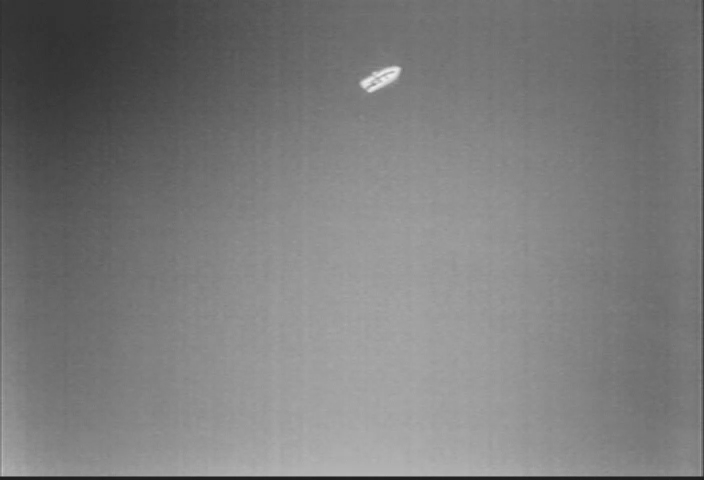
\includegraphics[width=\textwidth]{fig1}
		\caption{caption..}
		\label{fig:2a}
	\end{subfigure}
	~ %add desired spacing between images, e. g. ~, \quad, \qquad, \hfill etc.
	%(or a blank line to force the subfigure onto a new line)
	\begin{subfigure}[b]{0.45\textwidth}
		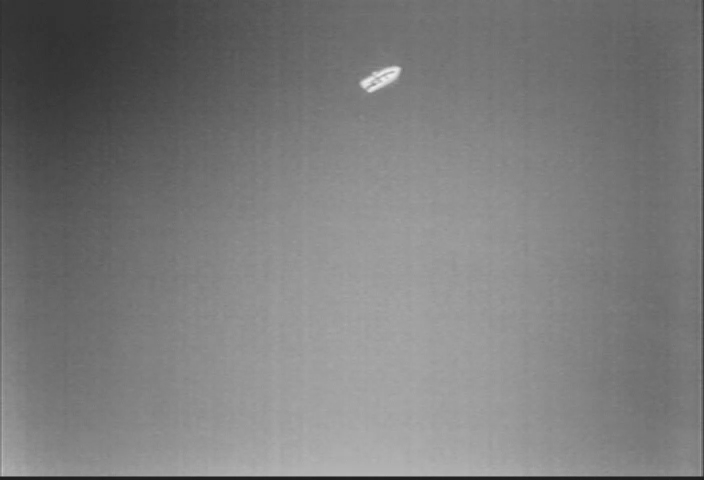
\includegraphics[width=\textwidth]{fig1}
		\caption{caption..}
		\label{fig:2b}
	\end{subfigure}
	\begin{subfigure}[b]{0.45\textwidth}
		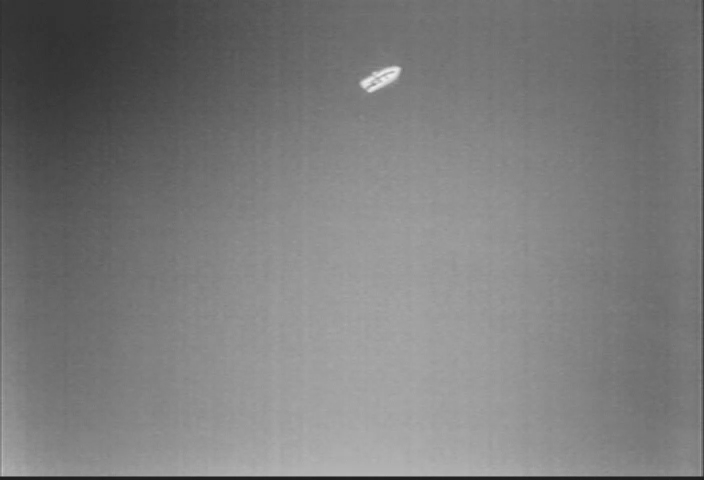
\includegraphics[width=\textwidth]{fig1}
		\caption{caption..}
		\label{fig:2c}
	\end{subfigure}
	\begin{subfigure}[b]{0.45\textwidth}
		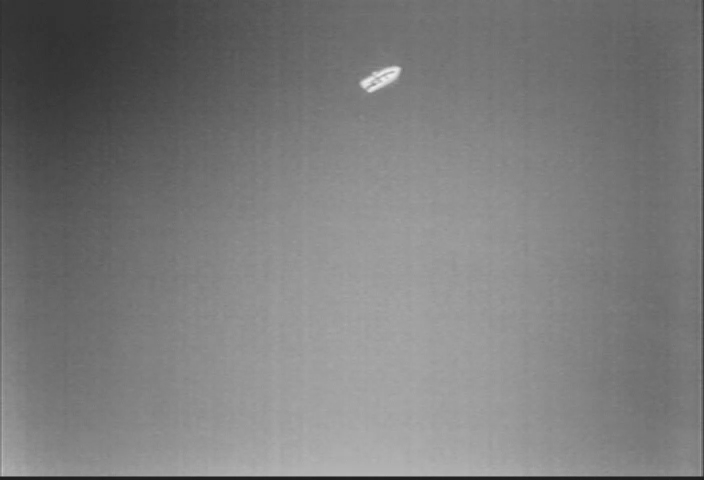
\includegraphics[width=\textwidth]{fig1}
		\caption{caption..}
		\label{fig:2d}
	\end{subfigure}
	\caption{Caption for all figures}\label{fig:2}
\end{figure}




